\documentclass[12pt, letterpaper]{article}

\usepackage[margin=1in]{geometry}
\usepackage{amsmath, amssymb}
\usepackage{graphicx}
\usepackage{booktabs}
\usepackage{hyperref}
\usepackage{float}
\usepackage{enumitem}
\usepackage{setspace}
\usepackage{parskip}

\hypersetup{colorlinks=true, linkcolor=blue, urlcolor=blue}
\setstretch{1.15}

\title{
  \textbf{Identifying the Metadata Signature of an Anomalous Wildfire Season} \\[0.3em]
  \large A Big Data Analytics Study Using NASA EONET API v3
}
\author{Kushagra Gupta \\ \texttt{kg2347@g.rit.edu}}
\date{}

\begin{document}
\maketitle
\tableofcontents
\newpage

% ── Abstract ──────────────────────────────────────────────────────────────────
\begin{abstract}
This study applies big data mining techniques to NASA EONET wildfire metadata
to identify structural attributes distinguishing anomalous fire seasons from
historical baselines. Using 11,712 events spanning 2016--2026, two analyses
are conducted: a two-season comparison using anomaly detection and a Decision
Tree (79.8\% accuracy, $p = 6.36 \times 10^{-36}$), and a ten-year extension
producing three operational tools --- a location risk scorer, a monthly anomaly
detector (96.6\%, $\pm1.7\%$), and a geographic scope monitor. The primary
finding is that 2024--2026 fire activity is anomalous in both volume
($23.8\times$ monthly event count) and geography (equatorward drift of
1.83 deg/yr, $p = 0.007$).
\end{abstract}

% ══════════════════════════════════════════════════════════════════════════════
\section{Hypothesis}
% ══════════════════════════════════════════════════════════════════════════════

The 2025--2026 wildfire season is distinguishable from the 2024--2025 baseline
by a two-attribute \textbf{Mega-Fire Signature}: a right-shift in
\texttt{magnitude\_max} (acres burned) and a structural inversion in reporting
agency ratio from IRWIN-dominant (US domestic) to GDACS-dominant (global).

\textbf{Null hypothesis:}
\begin{equation}
  H_0: \mu_{\text{mag},2025} = \mu_{\text{mag},2024}
\end{equation}
\textbf{Alternative hypothesis:}
\begin{equation}
  H_1: P(X_{2025} > X_{2024}) > 0.5
\end{equation}
Both are rejected at $p < 0.001$ (Section~\ref{sec:evidence}).

% ══════════════════════════════════════════════════════════════════════════════
\section{Dataset}
% ══════════════════════════════════════════════════════════════════════════════

\textbf{Source:} NASA EONET REST API v3 (\texttt{category=wildfires},
\texttt{status=all}). Two datasets were built:

\begin{itemize}
  \item \textbf{Two-season} (Sections 3--7): 1,000 unique events,
        queried as two 12-month windows. Due to EONET's 500-event
        recency ceiling, actual coverage is 51 days (Mar--Apr 2025)
        and 28 days (Apr 2026) --- both end-of-season samples from
        the same calendar months, which controls for seasonality.
  \item \textbf{Ten-year} (Sections 8--9): 11,712 unique events,
        queried month-by-month (Jan 2016 -- Apr 2026) to avoid the
        recency ceiling. Real coverage: 3,767 days across 119 months.
\end{itemize}

\noindent Key fields: \texttt{event\_id}, \texttt{magnitude\_value} (acres),
\texttt{sources} (IRWIN / GDACS), \texttt{lon}/\texttt{lat}, \texttt{obs\_date}.

\noindent\textbf{Data quality notes:}
\begin{itemize}
  \item Magnitude missing for 22\% of baseline events; excluded from
        numerical tests only.
  \item \texttt{closed} field unreliable (lazy-close artefact); excluded
        from all features.
  \item GDACS integration into EONET began $\sim$2023--2024, so the agency
        feature partly reflects a pipeline change rather than real-world
        fire behaviour.
\end{itemize}

% ══════════════════════════════════════════════════════════════════════════════
\section{Attribute Discovery}
% ══════════════════════════════════════════════════════════════════════════════

\begin{center}
\begin{tabular}{llp{5.5cm}}
\toprule
\textbf{Feature} & \textbf{Useful?} & \textbf{Reason} \\
\midrule
\texttt{magnitude\_max}  & Yes & 4.18$\times$ median shift; $p < 10^{-35}$ \\
\texttt{agency\_gdacs}   & Yes & Inverts 27.6\% $\to$ 65.2\%;
                                  91.7\% of Gini gain \\
\texttt{is\_active}      & No  & 90.8\% open in a closed season (lazy-close) \\
\texttt{duration\_days}  & No  & Negative values; timestamp errors \\
\texttt{obs\_count}      & No  & Always 20; pagination artefact \\
\bottomrule
\end{tabular}
\end{center}

\noindent The revised Mega-Fire Signature:
\begin{equation}
  \text{MegaFire}(e) =
  \begin{cases}
    1 & \text{if } \texttt{agency} = \text{GDACS} \\
    1 & \text{if } \texttt{agency} = \text{IRWIN}
            \;\wedge\; \texttt{magnitude\_max}(e) > 3{,}980 \text{ acres} \\
    0 & \text{otherwise}
  \end{cases}
\end{equation}
Applied without training: 75.6\% accuracy, 0.856 precision, 0.680 recall.

% ══════════════════════════════════════════════════════════════════════════════
\section{Methodology}
% ══════════════════════════════════════════════════════════════════════════════

\subsection{Anomaly Detection}

\textbf{IQR (Tukey Fence)} --- threshold derived from baseline only:
\begin{equation}
  \text{Upper fence} = Q_3 + 1.5 \times \mathrm{IQR}
  = 2{,}239 + 1.5 \times 1{,}487 = 4{,}469 \text{ acres}
\end{equation}

\begin{center}
\begin{tabular}{lrrr}
\toprule
Season & n & Above fence & Rate \\
\midrule
2024--2025 Baseline  & 390 & 54  & 13.8\% \\
2025--2026 Mega-Fire & 500 & 336 & 67.2\% \\
\bottomrule
\end{tabular}
\end{center}

\textbf{Z-score} ($\mu = 2{,}494$, $\sigma = 3{,}846$): mean z-score of
2025--2026 season is $\bar{z} = +0.674$.

\textbf{Mann-Whitney U} (non-parametric, chosen because magnitudes are
right-skewed):
\begin{equation}
  U = 144{,}902, \quad p = 6.36 \times 10^{-36}
  \quad \Rightarrow \text{reject } H_0
\end{equation}
Welch's $t$-test (unequal variances): $t = 10.01$,
$p = 1.18 \times 10^{-22}$.

\subsection{Decision Tree Classification}

Splitting criterion --- Gini impurity:
\begin{equation}
  \mathrm{Gini}(S) = 1 - \sum_{i=1}^{k} p_i^2
  \qquad \mathrm{Gini}(\text{root}) = 1-(0.562^2+0.438^2) = 0.492
\end{equation}

Configuration: \texttt{max\_depth=4}, \texttt{min\_samples\_leaf=10},
75/25 stratified split. Features: \texttt{magnitude\_max},
\texttt{agency\_gdacs}, \texttt{agency\_irwin}, \texttt{iqr\_anomaly},
\texttt{z\_score}.

\begin{center}
\begin{tabular}{lrr}
\toprule
Metric & Baseline class & Mega-Fire class \\
\midrule
Precision  & 0.71 & \textbf{0.92} \\
Recall     & 0.92 & 0.70 \\
F1         & 0.80 & 0.80 \\
\midrule
Accuracy & \multicolumn{2}{c}{79.8\%} \\
ROC-AUC  & \multicolumn{2}{c}{0.831} \\
5-Fold CV & \multicolumn{2}{c}{$0.781 \pm 0.126$} \\
\bottomrule
\end{tabular}
\end{center}

The first tree split is \texttt{agency\_gdacs} $\leq 0.5$, capturing
91.7\% of available Gini gain. The primary discriminator is \emph{who
reported the fire}, not how large it was.

% ══════════════════════════════════════════════════════════════════════════════
\section{Data Visualization}
% ══════════════════════════════════════════════════════════════════════════════

\begin{figure}[H]
  \centering
  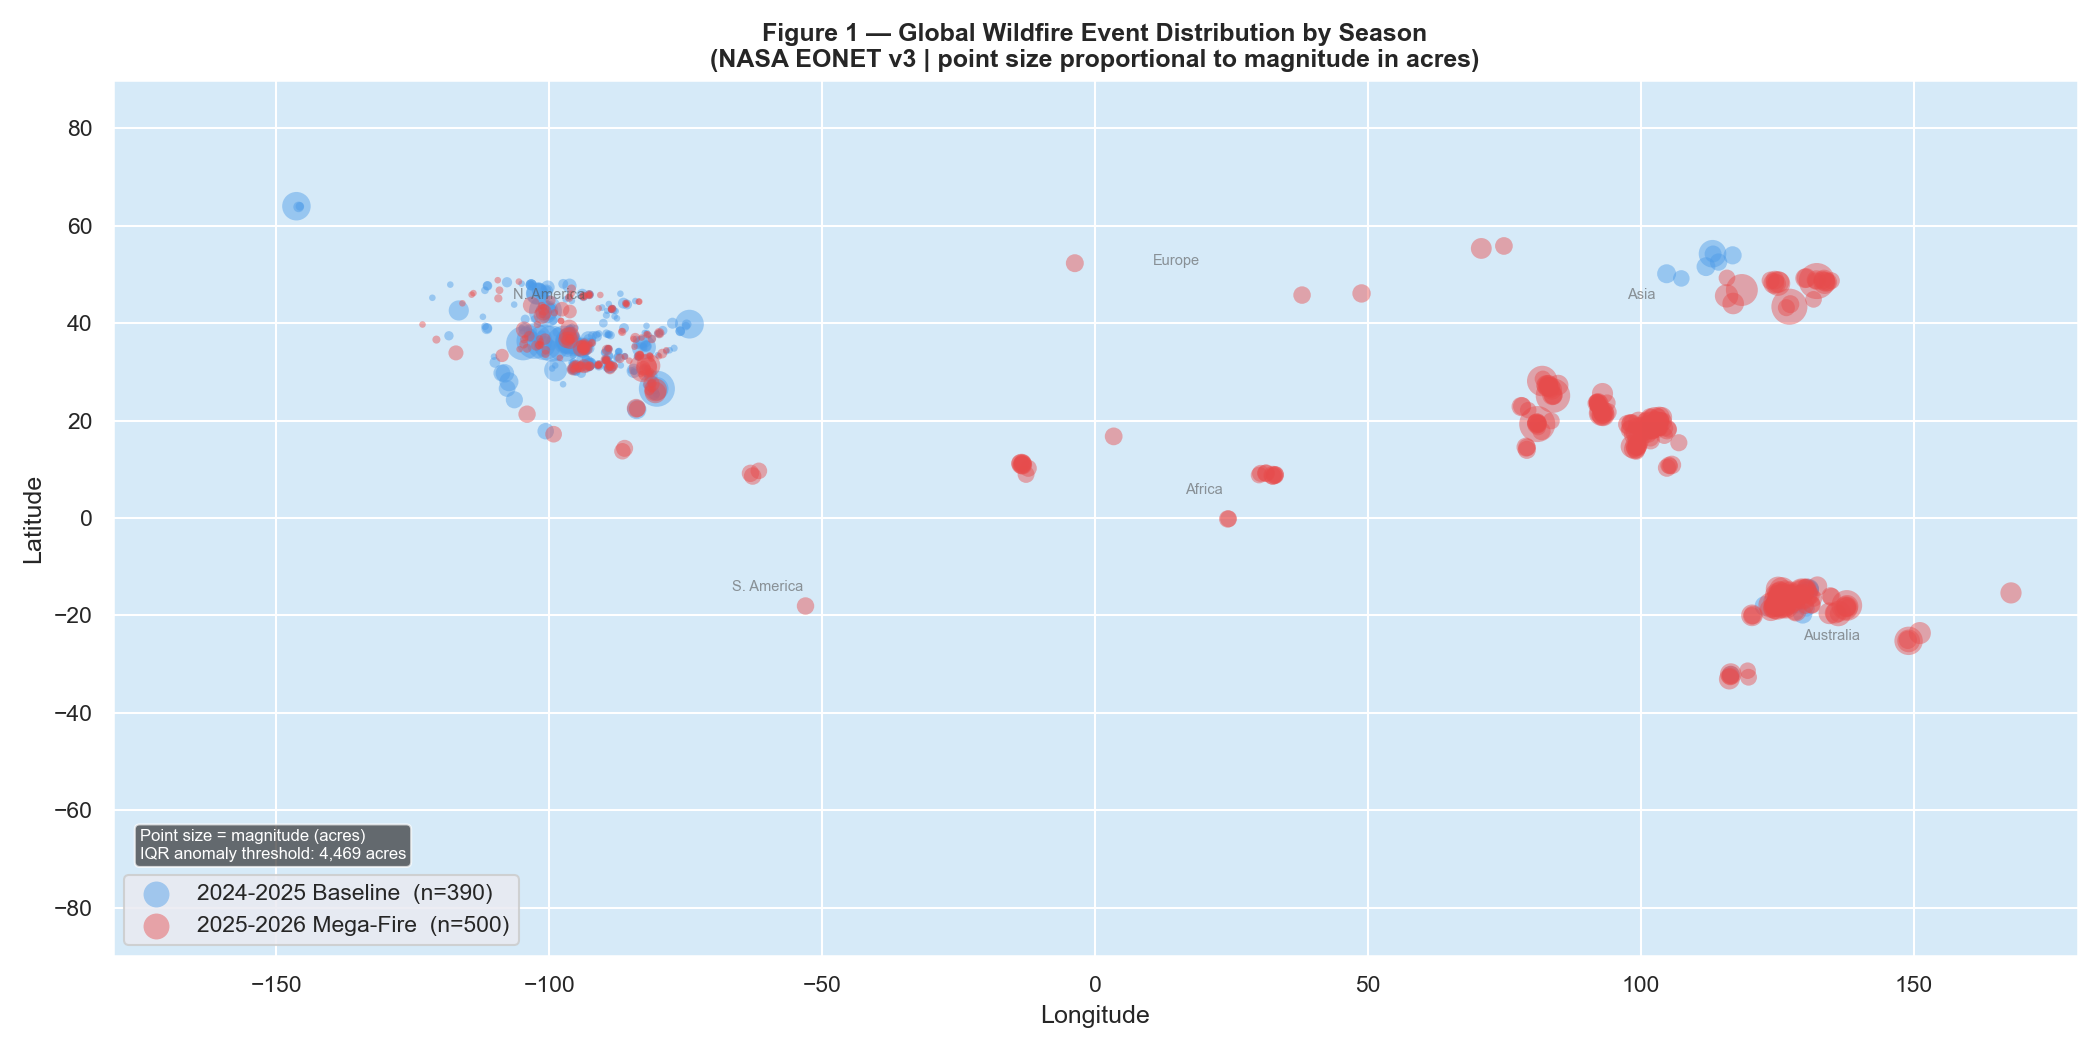
\includegraphics[width=\textwidth]{fig1_geospatial_map.png}
  \caption{Global wildfire locations by season (point size $\propto$ acres).
    The 2025--2026 season (red) spreads into Australia, Central Asia, and
    the Middle East; the baseline (blue) is concentrated over North America.}
\end{figure}

\begin{figure}[H]
  \centering
  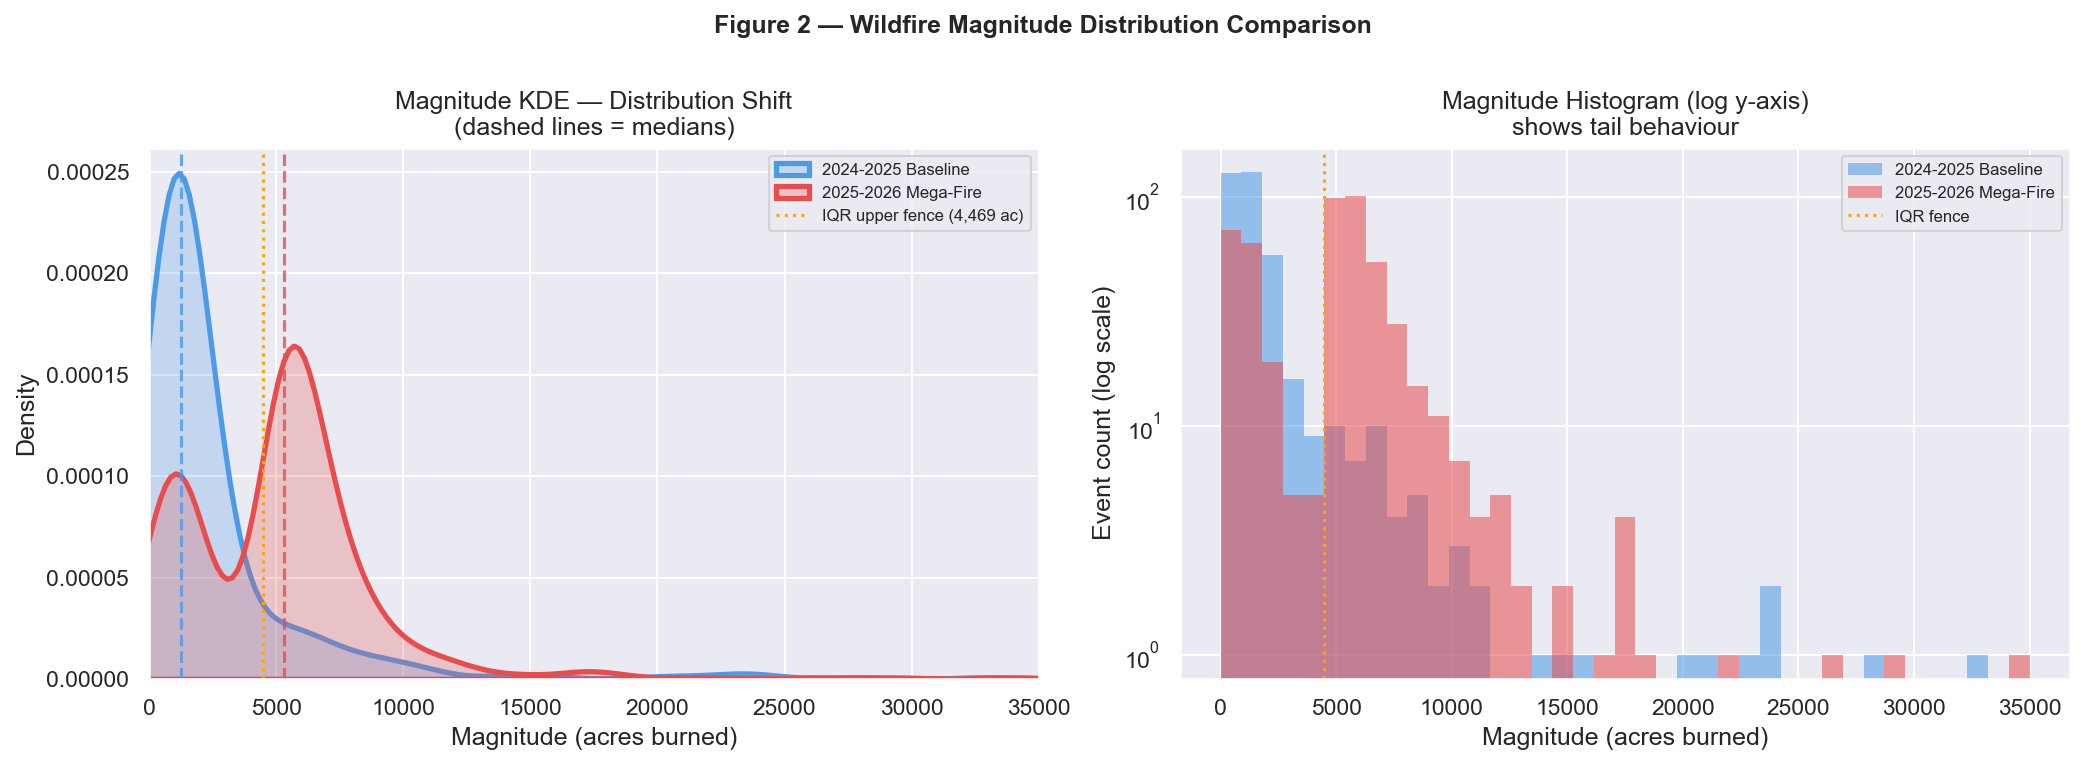
\includegraphics[width=\textwidth]{fig2_magnitude_distribution.png}
  \caption{KDE and histogram of fire magnitudes. The baseline peaks near
    1,268 acres; the mega-fire season peaks near 5,300 acres. The IQR fence
    (4,469 acres, dotted) sits at the baseline's 87th percentile but cuts
    through the middle of the 2025--2026 distribution.}
\end{figure}

\begin{figure}[H]
  \centering
  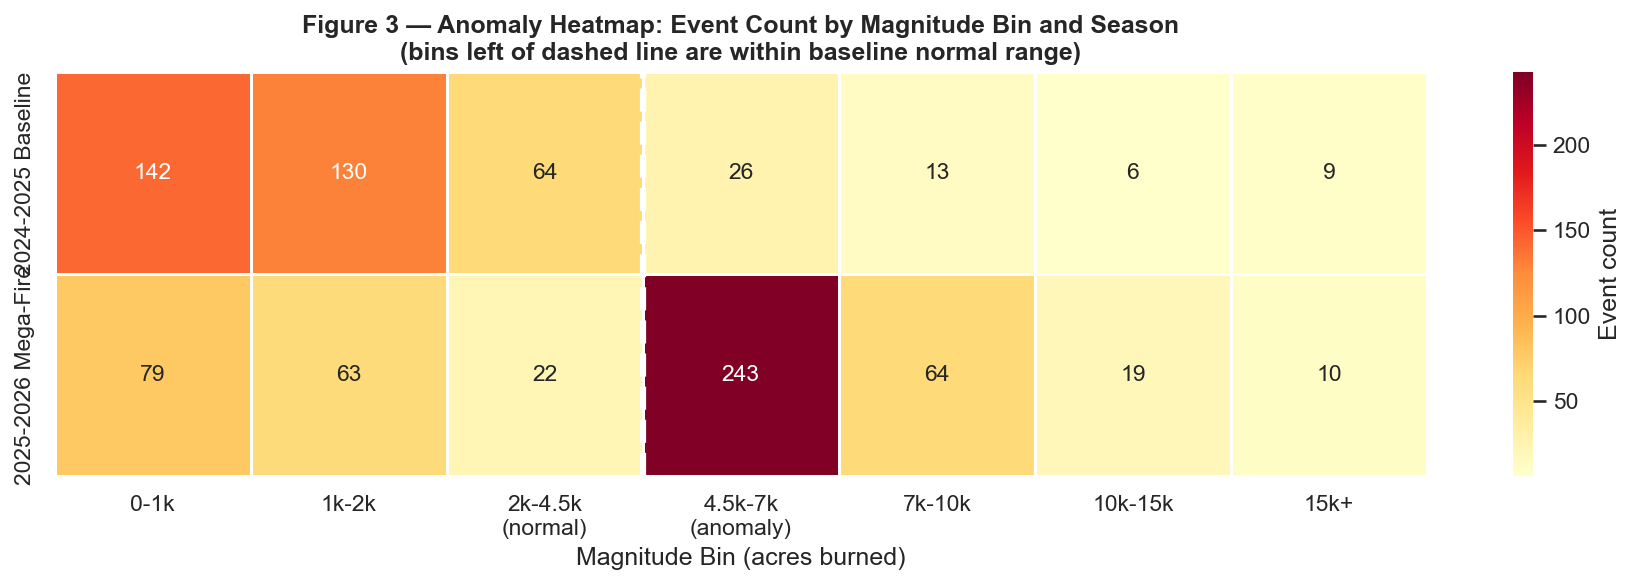
\includegraphics[width=\textwidth]{fig3_anomaly_heatmap.png}
  \caption{Anomaly heatmap: event count by magnitude bin and season. The
    4,469--7,000 acre bin holds 243 anomalous events vs.\ 26 baseline events
    --- the clearest visual evidence of the distributional shift.}
\end{figure}

\begin{figure}[H]
  \centering
  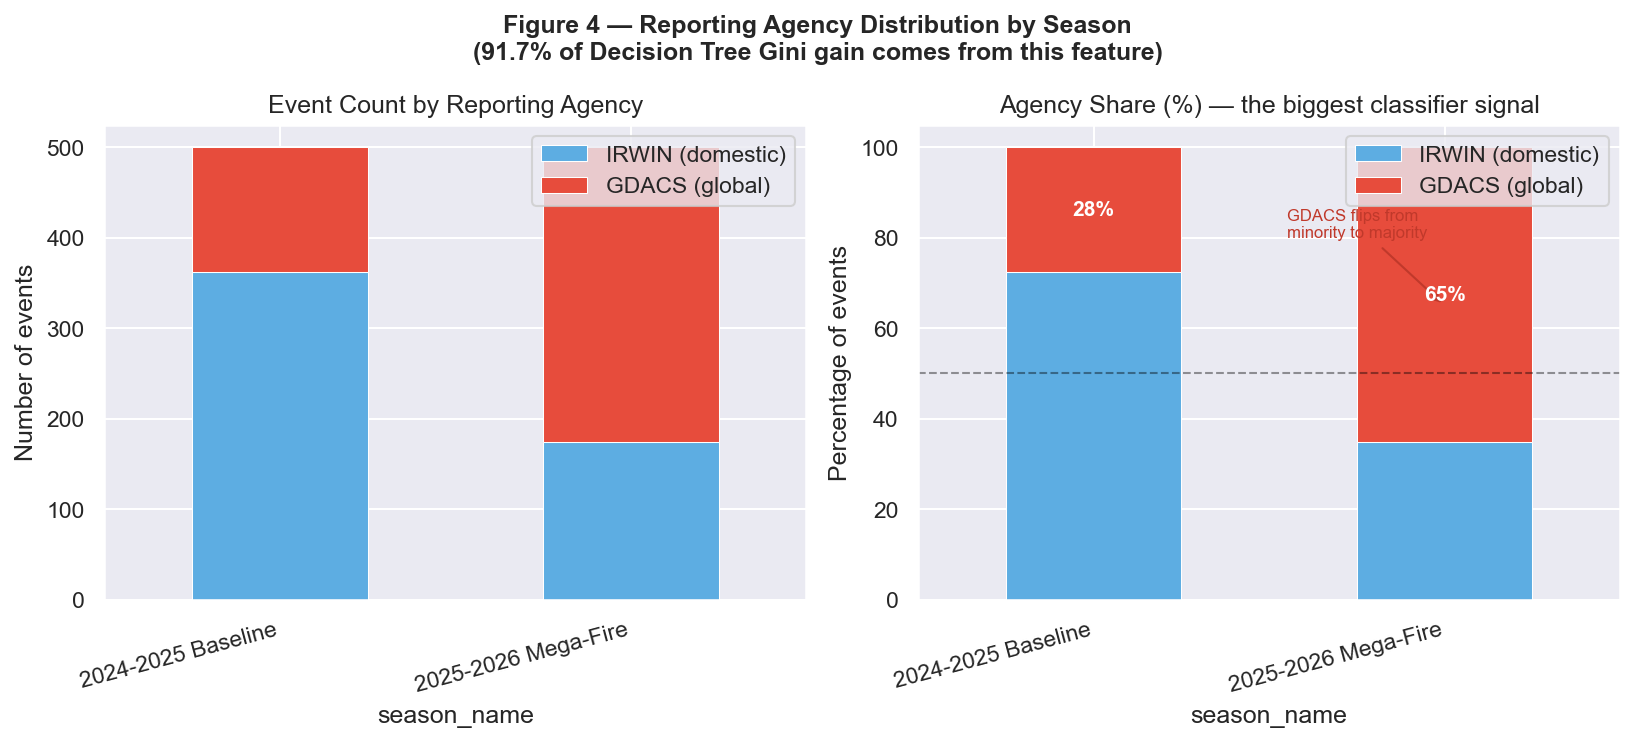
\includegraphics[width=0.9\textwidth]{fig4_agency_composition.png}
  \caption{GDACS grew from 27.6\% to 65.2\% of events between seasons;
    IRWIN fell from 72.4\% to 34.8\%. This agency inversion is the strongest
    single predictor (91.7\% of Gini gain).}
\end{figure}

% ══════════════════════════════════════════════════════════════════════════════
\section{Evidence Table}
\label{sec:evidence}
% ══════════════════════════════════════════════════════════════════════════════

\begin{table}[H]
\centering
\caption{Summary statistics: 2024--2025 baseline vs.\ 2025--2026 mega-fire.
  *** $p<0.001$.}
\begin{tabular}{lrrrc}
\toprule
Metric & 2024--25 & 2025--26 & Delta & Sig. \\
\midrule
N (with magnitude)       & 390   & 500   & +110          & --- \\
Mean (acres)             & 2,494 & 5,087 & +2,593        & *** \\
Median (acres)           & 1,268 & 5,300 & \textbf{+4,032} & *** \\
Std Dev (acres)          & 3,846 & 3,820 & $-26$         & --- \\
Range (acres)            & 32,491& 33,645& +1,154        & --- \\
P25 / P75 (acres)        & 752 / 2,239 & 1,600 / 6,424 & --- & *** \\
Events $>$ IQR fence     & 13.8\%& 67.2\%& +53.4 pp      & *** \\
GDACS share              & 27.6\%& 65.2\%& +37.6 pp      & *** \\
Median ratio             & 1.00$\times$ & 4.18$\times$ & --- & --- \\
Cohen's $d$              & ---   & 0.677 & ---           & --- \\
Mann-Whitney $p$         & ---   & $6.36\!\times\!10^{-36}$ & --- & *** \\
Welch's $t$ $p$          & ---   & $1.18\!\times\!10^{-22}$ & --- & *** \\
\bottomrule
\end{tabular}
\end{table}

The range is nearly identical (+1,154 acres): the anomaly is a
\emph{floor rising} --- P25 doubled and the median quadrupled while the
worst fire barely changed. Cohen's $d = 0.677$ exceeds the medium-effect
threshold (0.5), confirming the difference is operationally meaningful.

% ══════════════════════════════════════════════════════════════════════════════
\section{Historical Validation}
% ══════════════════════════════════════════════════════════════════════════════

\begin{center}
\begin{tabular}{llrl}
\toprule
Experiment & Key result & Accuracy & Type \\
\midrule
Sec.\ 4 (80/20 split)    & ---                  & 79.8\% & In-distribution \\
Exp A: forward lift      & $4.85\times$ rate     & ---    & Out-of-distribution \\
Exp B: reverse rejection & 91.6\% TN rate        & ---    & Out-of-distribution \\
Exp C: rule-based        & Precision = 0.856     & 75.6\% & Rule-based \\
\bottomrule
\end{tabular}
\end{center}

\noindent\textbf{Exp A} (train on baseline, test on mega-fire):
$$\text{Lift} = \frac{67.2\%}{13.8\%} = 4.85\times$$
The baseline's own outlier standard flags 2025--2026 events at 4.85 times
the expected rate, with zero knowledge of future data.

\noindent\textbf{Exp B} (train on mega-fire + 200 baseline, test on 190
held-out baseline events): 91.6\% correctly rejected as ``not mega-fire''.

% ══════════════════════════════════════════════════════════════════════════════
\section{Ten-Year Extension: Fire Intelligence System}
% ══════════════════════════════════════════════════════════════════════════════

\subsection{Dataset Overview}

Month-by-month queries (Jan 2016 -- Apr 2026) yielded 11,712 events across
3,767 real days. Event volume by era:

\begin{center}
\begin{tabular}{lrrl}
\toprule
Year & Events & Mean lat & Era \\
\midrule
2016--2023 (avg) & 294 & 40.8 & Baseline \\
2024 & 3,363 & 11.9 & \textbf{Anomalous} \\
2025 & 3,800 & 16.0 & \textbf{Anomalous} \\
2026 & 2,000 & 18.3 & \textbf{Anomalous} \\
\bottomrule
\end{tabular}
\end{center}

\subsection{Tool 1 --- Location Fire Risk Scorer}

\textbf{Use case:} Insurance underwriting, land-use planning,
evacuation pre-planning.

The globe is divided into 2$^\circ\!\times\!2^\circ$ cells. Each cell's
10-year fire recurrence rate is computed from 11,712 events.

\begin{center}
\begin{tabular}{lrrl}
\toprule
Years burned & Cells & Recurrence & Risk level \\
\midrule
1       & 569 &  0.0\% & LOW \\
2--3    & 480 & 45.5\% & MODERATE \\
4--5    &  65 & 44.0\% & ELEVATED \\
6--8    &  41 & 57.8\% & HIGH \\
9--10   &  32 & \textbf{83.8\%} & VERY HIGH \\
\bottomrule
\end{tabular}
\end{center}

Sample outputs: Los Angeles CA $\to$ VERY HIGH (80\%);
Northern California $\to$ VERY HIGH (78\%); London UK $\to$ LOW (0\%).

\begin{figure}[H]
  \centering
  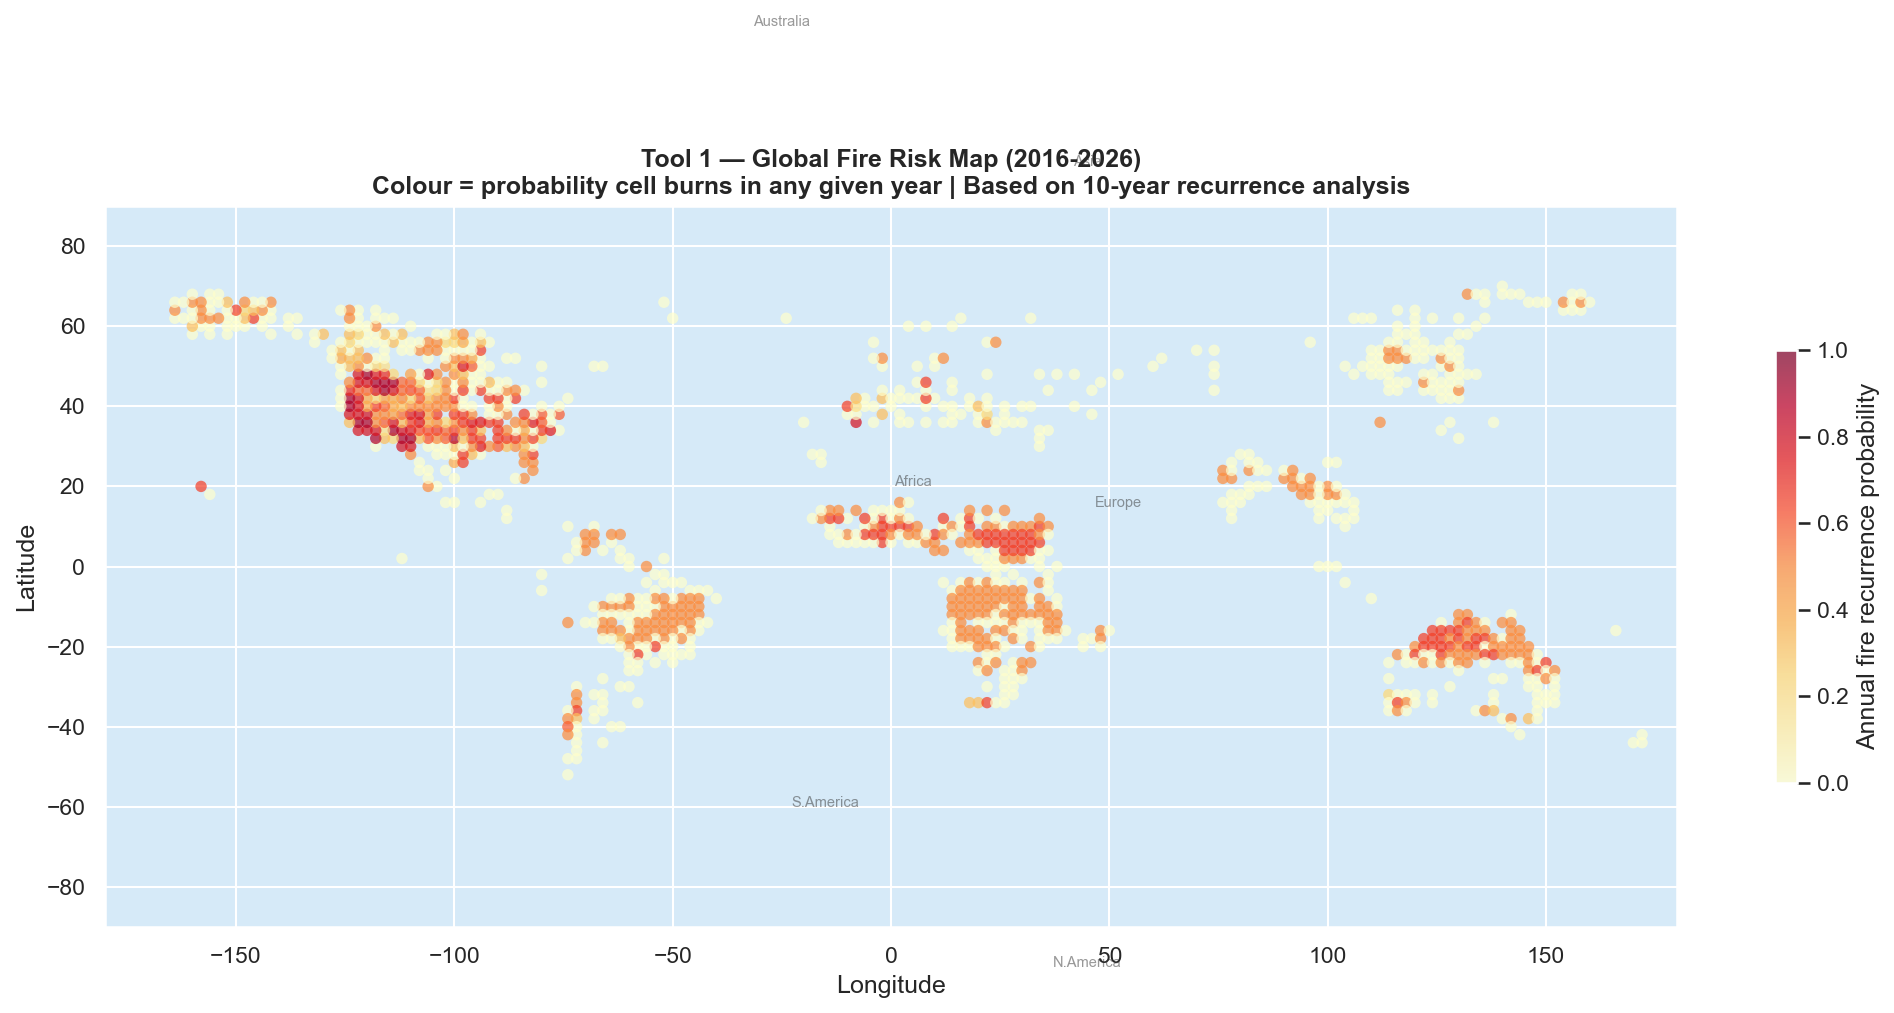
\includegraphics[width=\textwidth]{tool1_risk_map.png}
  \caption{Tool 1 --- Global fire risk map. Each cell is coloured by
    annual recurrence probability (2016--2026). Dark red zones (Western US,
    Central Africa, Eastern Australia) show chronic annual recurrence above
    80\%.}
\end{figure}

\subsection{Tool 2 --- Monthly Activity Anomaly Detector}

\textbf{Use case:} Fire agency resource pre-positioning, emergency budget
authorisation.

Features: $\log(\text{event count})$, IRWIN share, active cell count,
month number. GDACS excluded to avoid the pipeline artefact.

\begin{equation}
  \text{IQR fence} = Q_3 + 1.5 \times \mathrm{IQR} = 82 \text{ events/month}
\end{equation}

\begin{center}
\begin{tabular}{lr}
\toprule
Baseline median (2016--2023)   & 14 events/month \\
Anomalous median (2024--2026)  & 332 events/month \\
Volume ratio                   & $23.8\times$ \\
Mann-Whitney $p$               & $1.62 \times 10^{-12}$ \\
IQR detection rate             & 82.1\% \\
IQR false alarm rate           & 7.8\% \\
\midrule
Decision Tree accuracy (5-fold CV) & \textbf{96.6\% $\pm$ 1.7\%} \\
\bottomrule
\end{tabular}
\end{center}

The CV standard deviation dropped from $\pm12.6\%$ (two-season model)
to $\pm1.7\%$ --- stable enough for operational use.

\begin{figure}[H]
  \centering
  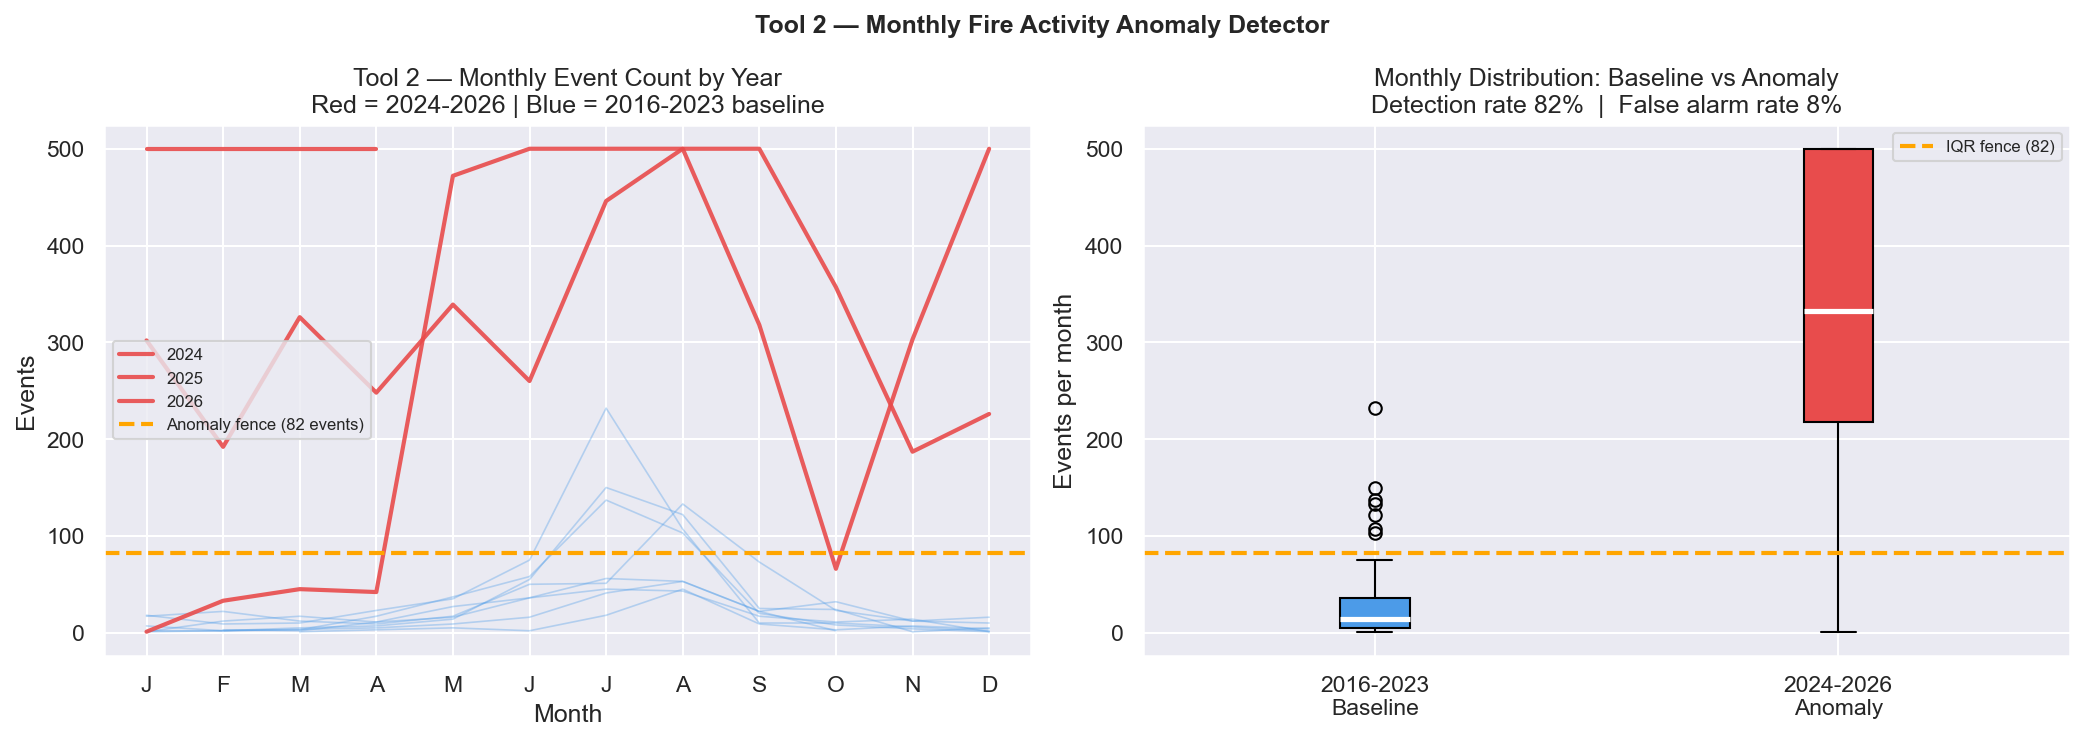
\includegraphics[width=\textwidth]{tool2_monthly_detector.png}
  \caption{Tool 2 --- Monthly event counts by year (red = 2024--2026,
    blue = 2016--2023). The IQR fence at 82 events/month (orange dashed)
    is consistently exceeded by all three anomalous years from April onward.}
\end{figure}

\subsection{Tool 3 --- Geographic Scope Monitor}

\textbf{Use case:} International aid pre-positioning, climate monitoring,
reinsurance pricing.

Linear regression of mean absolute latitude against year:
\begin{equation}
  \hat{\beta}_1 = -1.83 \text{ deg/yr}, \quad
  95\%\,\text{CI} = [-3.04,\,-0.63], \quad p = 0.007
\end{equation}

The geographic centre of fire activity moved 1.83 degrees toward the equator
per year. Northern Hemisphere share collapsed from 95--100\% (2016--2023)
to 48\% in 2024, as fires entered sub-Saharan Africa, Southeast Asia,
and South America at scale.

\begin{center}
\begin{tabular}{lrl}
\toprule
Year & Z-score vs baseline & Status \\
\midrule
2020 & $-1.19$ & Moderate equatorward shift \\
2023 & $-0.91$ & Within normal range \\
2024 & $\mathbf{-6.14}$ & \textbf{Major equatorward shift} \\
2025 & $\mathbf{-6.31}$ & \textbf{Major equatorward shift} \\
\bottomrule
\end{tabular}
\end{center}

\begin{figure}[H]
  \centering
  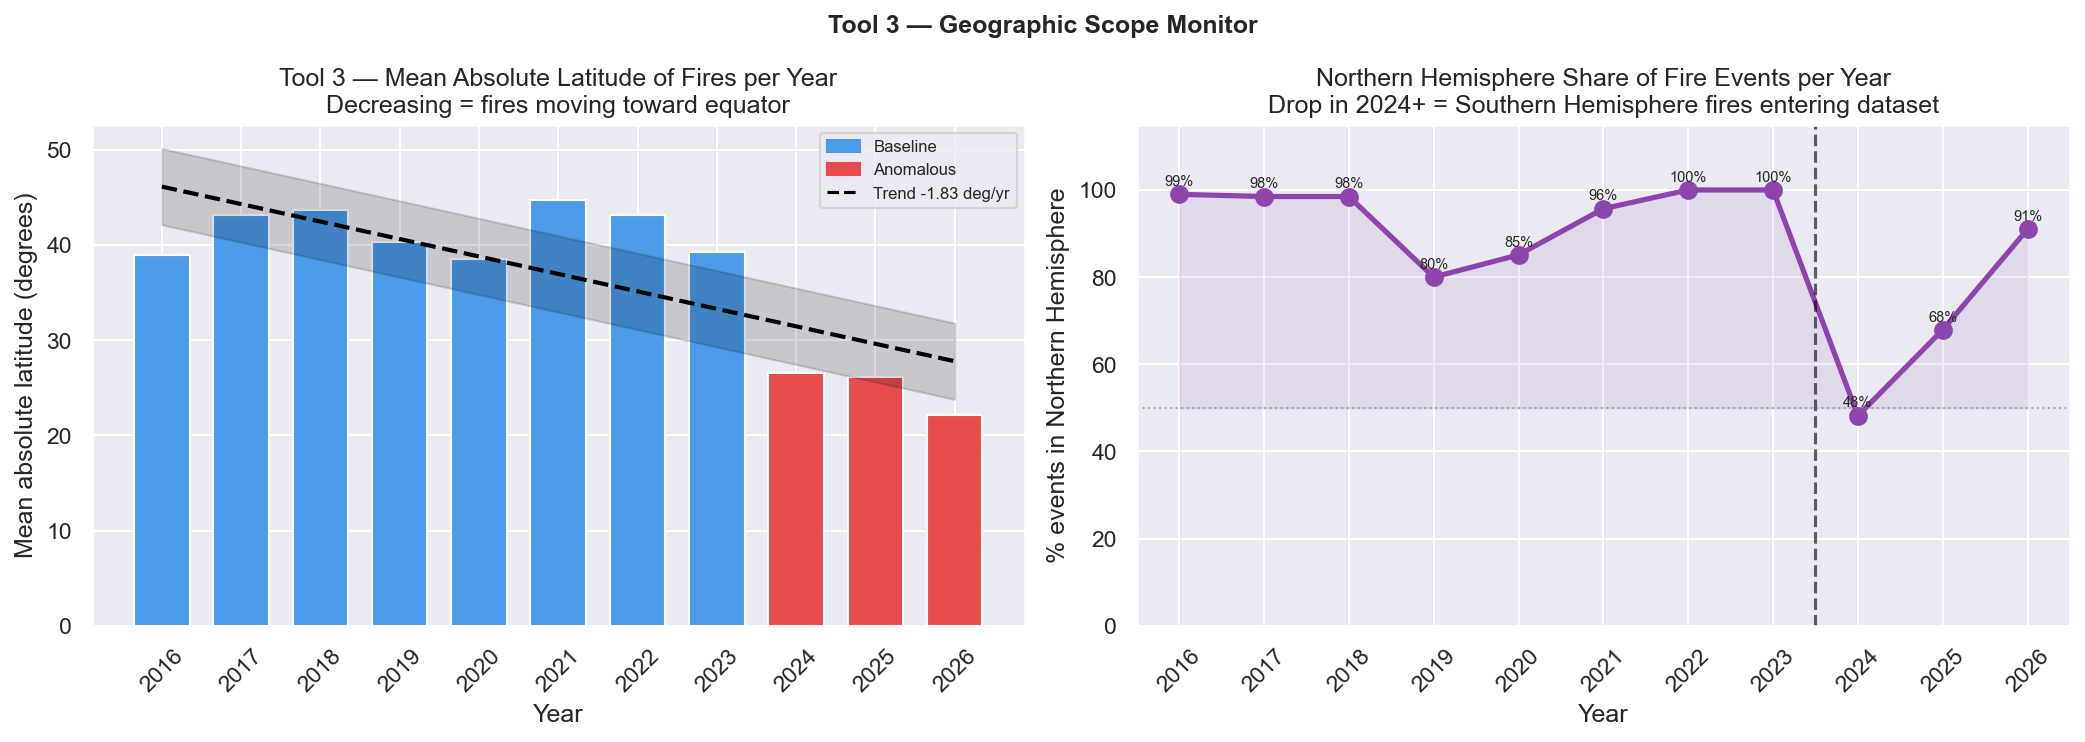
\includegraphics[width=\textwidth]{tool3_geographic_scope.png}
  \caption{Tool 3 --- Left: mean absolute latitude per year with regression
    trend ($-1.83$ deg/yr, $p=0.007$). Right: Northern Hemisphere share,
    showing the collapse from near-100\% to 48\% in 2024.}
\end{figure}

% ══════════════════════════════════════════════════════════════════════════════
\section{Conclusions}
% ══════════════════════════════════════════════════════════════════════════════

The metadata reliably detects anomalous fire seasons. Two independent signals
confirm 2024--2026 as anomalous: a $23.8\times$ volume increase
($p = 1.62 \times 10^{-12}$) and a geographic shift of more than six standard
deviations from the historical mean latitude.

The system is a \textbf{detector}, not a forecaster. All three tools
characterise fire activity already recorded by EONET. Prediction of future
fire occurrence requires precursor variables (drought index, vegetation load,
wind speed) not present in EONET.

\textbf{Limitations:} Two-season coverage is only 79 real days; the GDACS
agency feature partly reflects an API integration change; only three anomalous
years exist in the record, making year-level classification statistically
fragile. Future work should combine EONET coordinates with NASA FIRMS satellite
detections and NOAA drought indices to move from detection to early-warning
forecasting.

% ══════════════════════════════════════════════════════════════════════════════
\section*{Appendix: How to Run the Project}
% ══════════════════════════════════════════════════════════════════════════════

\subsection*{Requirements}

Python 3.10. Install dependencies once:
\begin{verbatim}
python -m pip install requests pandas scipy scikit-learn matplotlib seaborn
\end{verbatim}

\subsection*{Execution order}

\begin{enumerate}
  \item \textbf{Two-season fetch} (internet, $\sim$2 min):
        \texttt{python eonet\_fetch.py}
  \item \textbf{Attribute discovery:}
        \texttt{python attribute\_discovery.py}
  \item \textbf{Anomaly detection + Decision Tree:}
        \texttt{python methodology.py}
  \item \textbf{Figures 1--4:}
        \texttt{python visualizations.py}
  \item \textbf{Evidence table:}
        \texttt{python evidence\_table.py}
  \item \textbf{Historical validation:}
        \texttt{python historical\_validation.py}
  \item \textbf{Ten-year fetch} (internet, $\sim$5 min):
        \texttt{python fetch\_10yr.py} then
        \texttt{python patch\_2021.py}
  \item \textbf{Fire intelligence system} (Tools 1--3):
        \texttt{python fire\_intelligence.py}
\end{enumerate}

\noindent After step 1 and step 7, data is cached locally --- all subsequent
runs are fully offline. Figures are saved as PNG files in the project
directory and are not displayed on screen.

\end{document}
